%% bare_jrnl.tex
%% V1.4b
%% 2015/08/26
%% by Michael Shell
%% see http://www.michaelshell.org/
%% for current contact information.
%%
%% This is a skeleton file demonstrating the use of IEEEtran.cls
%% (requires IEEEtran.cls version 1.8b or later) with an IEEE
%% journal paper.
%%
%% Support sites:
%% http://www.michaelshell.org/tex/ieeetran/
%% http://www.ctan.org/pkg/ieeetran
%% and
%% http://www.ieee.org/

%%*************************************************************************
%% Legal Notice:
%% This code is offered as-is without any warranty either expressed or
%% implied; without even the implied warranty of MERCHANTABILITY or
%% FITNESS FOR A PARTICULAR PURPOSE! 
%% User assumes all risk.
%% In no event shall the IEEE or any contributor to this code be liable for
%% any damages or losses, including, but not limited to, incidental,
%% consequential, or any other damages, resulting from the use or misuse
%% of any information contained here.
%%
%% All comments are the opinions of their respective authors and are not
%% necessarily endorsed by the IEEE.
%%
%% This work is distributed under the LaTeX Project Public License (LPPL)
%% ( http://www.latex-project.org/ ) version 1.3, and may be freely used,
%% distributed and modified. A copy of the LPPL, version 1.3, is included
%% in the base LaTeX documentation of all distributions of LaTeX released
%% 2003/12/01 or later.
%% Retain all contribution notices and credits.
%% ** Modified files should be clearly indicated as such, including  **
%% ** renaming them and changing author support contact information. **
%%*************************************************************************


% *** Authors should verify (and, if needed, correct) their LaTeX system  ***
% *** with the testflow diagnostic prior to trusting their LaTeX platform ***
% *** with production work. The IEEE's font choices and paper sizes can   ***
% *** trigger bugs that do not appear when using other class files.       ***                          ***
% The testflow support page is at:
% http://www.michaelshell.org/tex/testflow/


\DocumentMetadata{pdfversion=2.0, pdfstandard=A-4}
\documentclass[journal]{IEEEtran}
%
% If IEEEtran.cls has not been installed into the LaTeX system files,
% manually specify the path to it like:
% \documentclass[journal]{../sty/IEEEtran}





% Some very useful LaTeX packages include:
% (uncomment the ones you want to load)


% *** MISC UTILITY PACKAGES ***
%
%\usepackage{ifpdf}
% Heiko Oberdiek's ifpdf.sty is very useful if you need conditional
% compilation based on whether the output is pdf or dvi.
% usage:
% \ifpdf
%   % pdf code
% \else
%   % dvi code
% \fi
% The latest version of ifpdf.sty can be obtained from:
% http://www.ctan.org/pkg/ifpdf
% Also, note that IEEEtran.cls V1.7 and later provides a builtin
% \ifCLASSINFOpdf conditional that works the same way.
% When switching from latex to pdflatex and vice-versa, the compiler may
% have to be run twice to clear warning/error messages.






% *** CITATION PACKAGES ***
%
\usepackage{bookmark}
\usepackage{cite}
% cite.sty was written by Donald Arseneau
% V1.6 and later of IEEEtran pre-defines the format of the cite.sty package
% \cite{} output to follow that of the IEEE. Loading the cite package will
% result in citation numbers being automatically sorted and properly
% "compressed/ranged". e.g., [1], [9], [2], [7], [5], [6] without using
% cite.sty will become [1], [2], [5]--[7], [9] using cite.sty. cite.sty's
% \cite will automatically add leading space, if needed. Use cite.sty's
% noadjust option (cite.sty V3.8 and later) if you want to turn this off
% such as if a citation ever needs to be enclosed in parenthesis.
% cite.sty is already installed on most LaTeX systems. Be sure and use
% version 5.0 (2009-03-20) and later if using hyperref.sty.
% The latest version can be obtained at:
% http://www.ctan.org/pkg/cite
% The documentation is contained in the cite.sty file itself.



\usepackage{gensymb}


% *** GRAPHICS RELATED PACKAGES ***
%
\ifCLASSINFOpdf
  \usepackage[pdftex]{graphicx}
  % declare the path(s) where your graphic files are
  % \graphicspath{{../pdf/}{../jpeg/}}
  % and their extensions so you won't have to specify these with
  % every instance of \includegraphics
  % \DeclareGraphicsExtensions{.pdf,.jpeg,.png}
\else
  % or other class option (dvipsone, dvipdf, if not using dvips). graphicx
  % will default to the driver specified in the system graphics.cfg if no
  % driver is specified.
  \usepackage[dvips]{graphicx}
  % declare the path(s) where your graphic files are
  % \graphicspath{{../eps/}}
  % and their extensions so you won't have to specify these with
  % every instance of \includegraphics
  % \DeclareGraphicsExtensions{.eps}
\fi
\usepackage{xcolor,colorspace}
\usepackage{tikz}
\usepackage[]{circuitikz}
\usepackage{environ}
\makeatletter
\newsavebox{\measure@tikzpicture}
\NewEnviron{scaletikzpicturetowidth}[1]{%
  \def\tikz@width{#1}%
  \def\tikzscale{1}\begin{lrbox}{\measure@tikzpicture}%
  \BODY
  \end{lrbox}%
  \pgfmathparse{#1/\wd\measure@tikzpicture}%
  \edef\tikzscale{\pgfmathresult}%
  \BODY
}
\makeatother
\usepackage{pgfplots}
\usepackage{pgfplotstable}
\pgfplotsset{compat = newest}
\pgfplotsset{
  every axis legend/.append style =
    {
      % Change the text alignment so the end of the text (rather than the
      % start) lines up.
      cells = { anchor = east },
      % The standard pgfplots settings use a box around legends:
      % I prefer without this.
      draw  = none
    }
}
\pgfplotsset{
  myplot/.style =
    {
      % Using a cycle list just altering colour means that there are no
      % marks: that is normal for this sort of plot.
      cycle list name = color list , 
      % Ensure that the x-axis values always have the same number of 
      % decimal places, to avoid e.g. "1" but "1.2".
      every x tick label/.append style  =
        { 
          /pgf/number format/.cd ,
           precision = 1 , 
           fixed         ,
           zerofill
        },
      % The labels apply to all plots of this type.
      % Notice that in this case the zero is ferrocenium/ferrocene, but that
      % will depend on the experiment.
      xlabel = \(V_{CC}~(V)\),
      % The normalised y-axis has something of a nightmare label!
      ylabel = \(V_{ref}~(V)\),
    },
}
\makeatletter
\pgfplotsset{ % Tufte-like plot
  tufte axes/.style =
    {
      after end axis/.code =
        {
          \draw ({rel axis cs:0,0} -| {axis cs:\pgfplots@data@xmin,0})
            -- ({rel axis cs:0,0}  -| {axis cs:\pgfplots@data@xmax,0});
          \draw ({rel axis cs:0,0} |- {axis cs:0,\pgfplots@data@ymin})
            -- ({rel axis cs:0,0}  |-{axis cs:0,\pgfplots@data@ymax});
        },
      axis line style = {draw = none},
      tick align      = outside,
      tick pos        = left
    }
}
\makeatother
% \usepackage{pgfplots}
% \pgfplotsset{compat = newest}

% graphicx was written by David Carlisle and Sebastian Rahtz. It is
% required if you want graphics, photos, etc. graphicx.sty is already
% installed on most LaTeX systems. The latest version and documentation
% can be obtained at: 
% http://www.ctan.org/pkg/graphicx
% Another good source of documentation is "Using Imported Graphics in
% LaTeX2e" by Keith Reckdahl which can be found at:
% http://www.ctan.org/pkg/epslatex
%
% latex, and pdflatex in dvi mode, support graphics in encapsulated
% postscript (.eps) format. pdflatex in pdf mode supports graphics
% in .pdf, .jpeg, .png and .mps (metapost) formats. Users should ensure
% that all non-photo figures use a vector format (.eps, .pdf, .mps) and
% not a bitmapped formats (.jpeg, .png). The IEEE frowns on bitmapped formats
% which can result in "jaggedy"/blurry rendering of lines and letters as
% well as large increases in file sizes.
%
% You can find documentation about the pdfTeX application at:
% http://www.tug.org/applications/pdftex





% *** MATH PACKAGES ***
%
\usepackage{amsmath}
\usepackage{mathtools} % loads amsmath and fixes its bugs, empheq, etc
\usepackage{amssymb}
\usepackage{sympytex}
\usepackage{siunitx}
\sisetup{detect-all=true}   % ensure proper font weight
\sisetup{per-mode = repeated-symbol}    % ensure "/" unit delineator
\sisetup{range-phrase = --,range-units = brackets} % hyphenated ranges, SI syntax
\DeclareMathSymbol{\varOmega}{\mathalpha}{operators}{"0A}   % upright omega for ohms
\providecommand*{\Ohm}{\varOmega}   % for siunitx
\DeclareSIUnit\sq{\ensuremath{\Box}}    % sheet resistance
\DeclareSIUnit{\Siemens}{S}
\DeclareSIUnit{\torr}{Torr} % add torr to siunitix 3
\DeclareSIUnit\sig{\ensuremath{\sigma}}
\DeclareSIUnit\ppm{ppm}
\usepackage{xfrac}
% A popular package from the American Mathematical Society that provides
% many useful and powerful commands for dealing with mathematics.
%
% Note that the amsmath package sets \interdisplaylinepenalty to 10000
% thus preventing page breaks from occurring within multiline equations. Use:
%\interdisplaylinepenalty=2500
% after loading amsmath to restore such page breaks as IEEEtran.cls normally
% does. amsmath.sty is already installed on most LaTeX systems. The latest
% version and documentation can be obtained at:
% http://www.ctan.org/pkg/amsmath





% *** SPECIALIZED LIST PACKAGES ***
%
%\usepackage{algorithmic}
% algorithmic.sty was written by Peter Williams and Rogerio Brito.
% This package provides an algorithmic environment fo describing algorithms.
% You can use the algorithmic environment in-text or within a figure
% environment to provide for a floating algorithm. Do NOT use the algorithm
% floating environment provided by algorithm.sty (by the same authors) or
% algorithm2e.sty (by Christophe Fiorio) as the IEEE does not use dedicated
% algorithm float types and packages that provide these will not provide
% correct IEEE style captions. The latest version and documentation of
% algorithmic.sty can be obtained at:
% http://www.ctan.org/pkg/algorithms
% Also of interest may be the (relatively newer and more customizable)
% algorithmicx.sty package by Szasz Janos:
% http://www.ctan.org/pkg/algorithmicx




% *** ALIGNMENT PACKAGES ***
%
%\usepackage{array}
% Frank Mittelbach's and David Carlisle's array.sty patches and improves
% the standard LaTeX2e array and tabular environments to provide better
% appearance and additional user controls. As the default LaTeX2e table
% generation code is lacking to the point of almost being broken with
% respect to the quality of the end results, all users are strongly
% advised to use an enhanced (at the very least that provided by array.sty)
% set of table tools. array.sty is already installed on most systems. The
% latest version and documentation can be obtained at:
% http://www.ctan.org/pkg/array


% IEEEtran contains the IEEEeqnarray family of commands that can be used to
% generate multiline equations as well as matrices, tables, etc., of high
% quality.




% *** SUBFIGURE PACKAGES ***
\ifCLASSOPTIONcompsoc
  \usepackage[caption=false,font=normalsize,labelfont=sf,textfont=sf]{subfig}
\else
  \usepackage[caption=false,font=footnotesize]{subfig}
\fi
% subfig.sty, written by Steven Douglas Cochran, is the modern replacement
% for subfigure.sty, the latter of which is no longer maintained and is
% incompatible with some LaTeX packages including fixltx2e. However,
% subfig.sty requires and automatically loads Axel Sommerfeldt's caption.sty
% which will override IEEEtran.cls' handling of captions and this will result
% in non-IEEE style figure/table captions. To prevent this problem, be sure
% and invoke subfig.sty's "caption=false" package option (available since
% subfig.sty version 1.3, 2005/06/28) as this is will preserve IEEEtran.cls
% handling of captions.
% Note that the Computer Society format requires a larger sans serif font
% than the serif footnote size font used in traditional IEEE formatting
% and thus the need to invoke different subfig.sty package options depending
% on whether compsoc mode has been enabled.
%
% The latest version and documentation of subfig.sty can be obtained at:
% http://www.ctan.org/pkg/subfig




% *** FLOAT PACKAGES ***
%
%\usepackage{fixltx2e}
% fixltx2e, the successor to the earlier fix2col.sty, was written by
% Frank Mittelbach and David Carlisle. This package corrects a few problems
% in the LaTeX2e kernel, the most notable of which is that in current
% LaTeX2e releases, the ordering of single and double column floats is not
% guaranteed to be preserved. Thus, an unpatched LaTeX2e can allow a
% single column figure to be placed prior to an earlier double column
% figure.
% Be aware that LaTeX2e kernels dated 2015 and later have fixltx2e.sty's
% corrections already built into the system in which case a warning will
% be issued if an attempt is made to load fixltx2e.sty as it is no longer
% needed.
% The latest version and documentation can be found at:
% http://www.ctan.org/pkg/fixltx2e


\usepackage{stfloats}
% stfloats.sty was written by Sigitas Tolusis. This package gives LaTeX2e
% the ability to do double column floats at the bottom of the page as well
% as the top. (e.g., "\begin{figure*}[!b]" is not normally possible in
% LaTeX2e). It also provides a command:
%\fnbelowfloat
% to enable the placement of footnotes below bottom floats (the standard
% LaTeX2e kernel puts them above bottom floats). This is an invasive package
% which rewrites many portions of the LaTeX2e float routines. It may not work
% with other packages that modify the LaTeX2e float routines. The latest
% version and documentation can be obtained at:
% http://www.ctan.org/pkg/stfloats
% Do not use the stfloats baselinefloat ability as the IEEE does not allow
% \baselineskip to stretch. Authors submitting work to the IEEE should note
% that the IEEE rarely uses double column equations and that authors should try
% to avoid such use. Do not be tempted to use the cuted.sty or midfloat.sty
% packages (also by Sigitas Tolusis) as the IEEE does not format its papers in
% such ways.
% Do not attempt to use stfloats with fixltx2e as they are incompatible.
% Instead, use Morten Hogholm'a dblfloatfix which combines the features
% of both fixltx2e and stfloats:
%
% \usepackage{dblfloatfix}
% The latest version can be found at:
% http://www.ctan.org/pkg/dblfloatfix




%\ifCLASSOPTIONcaptionsoff
%  \usepackage[nomarkers]{endfloat}
% \let\MYoriglatexcaption\caption
% \renewcommand{\caption}[2][\relax]{\MYoriglatexcaption[#2]{#2}}
%\fi
% endfloat.sty was written by James Darrell McCauley, Jeff Goldberg and 
% Axel Sommerfeldt. This package may be useful when used in conjunction with 
% IEEEtran.cls'  captionsoff option. Some IEEE journals/societies require that
% submissions have lists of figures/tables at the end of the paper and that
% figures/tables without any captions are placed on a page by themselves at
% the end of the document. If needed, the draftcls IEEEtran class option or
% \CLASSINPUTbaselinestretch interface can be used to increase the line
% spacing as well. Be sure and use the nomarkers option of endfloat to
% prevent endfloat from "marking" where the figures would have been placed
% in the text. The two hack lines of code above are a slight modification of
% that suggested by in the endfloat docs (section 8.4.1) to ensure that
% the full captions always appear in the list of figures/tables - even if
% the user used the short optional argument of \caption[]{}.
% IEEE papers do not typically make use of \caption[]'s optional argument,
% so this should not be an issue. A similar trick can be used to disable
% captions of packages such as subfig.sty that lack options to turn off
% the subcaptions:
% For subfig.sty:
% \let\MYorigsubfloat\subfloat
% \renewcommand{\subfloat}[2][\relax]{\MYorigsubfloat[]{#2}}
% However, the above trick will not work if both optional arguments of
% the \subfloat command are used. Furthermore, there needs to be a
% description of each subfigure *somewhere* and endfloat does not add
% subfigure captions to its list of figures. Thus, the best approach is to
% avoid the use of subfigure captions (many IEEE journals avoid them anyway)
% and instead reference/explain all the subfigures within the main caption.
% The latest version of endfloat.sty and its documentation can obtained at:
% http://www.ctan.org/pkg/endfloat
%
% The IEEEtran \ifCLASSOPTIONcaptionsoff conditional can also be used
% later in the document, say, to conditionally put the References on a 
% page by themselves.
\usepackage{fontspec}
\setmainfont{STIXTwoText}[
	Extension		= .otf,
	UprightFont		= *-Regular,
	BoldFont		= *-Bold.otf,
	ItalicFont		= *-MediumItalic.otf,
	BoldItalicFont 	= *-BoldItalic.otf
]
\usepackage[math-style=ISO]{unicode-math}
\setmathfont{STIXTwoMath-Regular.otf} % for symbols
\usepackage{microtype}
\UseMicrotypeSet[protrusion]{basicmath} % disable protrusion for tt fonts
\urlstyle{same}
\newcommand{\unifrac}[2]{\mbox{% making sure we don't get a line break
    {\addfontfeatures{RawFeature=+numr}#1}%
    ⁄% That slash is U+2044 FRACTION SLASH, which has special spacing
    {\addfontfeatures{RawFeature=+dnom}#2}%
    }}



% *** PDF, URL AND HYPERLINK PACKAGES ***
%
%\usepackage{url}
% url.sty was written by Donald Arseneau. It provides better support for
% handling and breaking URLs. url.sty is already installed on most LaTeX
% systems. The latest version and documentation can be obtained at:
% http://www.ctan.org/pkg/url
% Basically, \url{my_url_here}.
\usepackage{orcidlink}
\RequirePackage[type={CC},modifier={by-nc-nd},version={4.0},lang={english}]{doclicense}

\usepackage{datetime2} % to satisfy the "\today" in \hypersetup
\DTMusemodule{english}{en-US}
\usepackage{hyperref}
\hypersetup{
    hyperindex=true,
    colorlinks=true,
	bookmarksnumbered,
    bookmarksopen=true,
    linkcolor=blue,
    filecolor=magenta,      
    urlcolor=cyan,
%%%%%%%%%%%%%%%% METADATA %%%%%%%%%%%%%%%%%%%%	
    pdftitle={EE726 Midterm},
	pdfsubject={Banba et al. Sub-1-V CMOS Bandgap Reference},
    pdfauthor={Chris Biancone},
	pdfpublisher={Chris Biancone},
	pdfkeywords={bandgap, voltage reference},
%%%%%%%%%%%%%%%%%%%%%%%%%%%%%%%%%%%%%%%%%%%%%%
	pdfproducer=luaLaTeX-1.17.0,
	pdfdate=\today,
	pdflang={en},pdfmetalang={en},
	pdflicenseurl={},
    pdfpagemode=FullScreen,
}
\usepackage[nameinlink,capitalize]{cleveref}
\newcommand*{\doi}{}
\makeatletter
\newcommand{\doi@}[1]{\href{https://doi.org/#1}{#1}}
\DeclareRobustCommand{\doi}{\hyper@normalise\doi@}
\makeatother


% *** Do not adjust lengths that control margins, column widths, etc. ***
% *** Do not use packages that alter fonts (such as pslatex).         ***
% There should be no need to do such things with IEEEtran.cls V1.6 and later.
% (Unless specifically asked to do so by the journal or conference you plan
% to submit to, of course. )


% correct bad hyphenation here
\hyphenation{op-tical net-works semi-conduc-tor}


\begin{document}
%
% paper title
% Titles are generally capitalized except for words such as a, an, and, as,
% at, but, by, for, in, nor, of, on, or, the, to and up, which are usually
% not capitalized unless they are the first or last word of the title.
% Linebreaks \\ can be used within to get better formatting as desired.
% Do not put math or special symbols in the title.
\title{Review of Sub-\qty{1}{\V} CMOS Bandgap References}
%
%
% author names and IEEE memberships
% note positions of commas and nonbreaking spaces ( ~ ) LaTeX will not break
% a structure at a ~ so this keeps an author's name from being broken across
% two lines.
% use \thanks{} to gain access to the first footnote area
% a separate \thanks must be used for each paragraph as LaTeX2e's \thanks
% was not built to handle multiple paragraphs
%

\author{Chris~Biancone,~\IEEEmembership{Member,~IEEE~\orcidlink{0009-0007-8759-4858}}
        
\thanks{C. Biancone is with the Department
of Electrical and Microelectronic Engineering, Rochester Institute of Technology, Rochester,
NY, 14623 USA e-mail: \href{mailto:cjb1402@rit.edu}{cjb1402@rit.edu}.}% <-this % stops a space

\thanks{Manuscript received Mar. 05, 2024}
}

% note the % following the last \IEEEmembership and also \thanks - 
% these prevent an unwanted space from occurring between the last author name
% and the end of the author line. i.e., if you had this:
% 
% \author{....lastname \thanks{...} \thanks{...} }
%                     ^------------^------------^----Do not want these spaces!
%
% a space would be appended to the last name and could cause every name on that
% line to be shifted left slightly. This is one of those "LaTeX things". For
% instance, "\textbf{A} \textbf{B}" will typeset as "A B" not "AB". To get
% "AB" then you have to do: "\textbf{A}\textbf{B}"
% \thanks is no different in this regard, so shield the last } of each \thanks
% that ends a line with a % and do not let a space in before the next \thanks.
% Spaces after \IEEEmembership other than the last one are OK (and needed) as
% you are supposed to have spaces between the names. For what it is worth,
% this is a minor point as most people would not even notice if the said evil
% space somehow managed to creep in.



% The paper headers
\markboth{Mixed-Signal IC Design, 2024}%
{Biancone, C. 2024}
% The only time the second header will appear is for the odd numbered pages
% after the title page when using the twoside option.
% 
% *** Note that you probably will NOT want to include the author's ***
% *** name in the headers of peer review papers.                   ***
% You can use \ifCLASSOPTIONpeerreview for conditional compilation here if
% you desire.




% If you want to put a publisher's ID mark on the page you can do it like
% this:
%\IEEEpubid{0000--0000/00\$00.00~\copyright~2015 IEEE}
% Remember, if you use this you must call \IEEEpubidadjcol in the second
% column for its text to clear the IEEEpubid mark.



% use for special paper notices
%\IEEEspecialpapernotice{(Invited Paper)}




% make the title area
\maketitle

% As a general rule, do not put math, special symbols or citations
% in the abstract or keywords.
\begin{abstract}
The continued push for lower supply voltages to VLSI circuits for reduced power consumption has led to a necessary adaptation for precision reference circuits. A bandgap reference circuit proposed by Banba et al. in 1998 is reviewed from its subsequent publication in 1999. This design adopts the current-mode method of generating a reference voltage, and by reconfiguring elements of a conventional design at the time, is adapted to operation under \qty{1}{\V} supply. This design has served as a foundation for countless low voltage bandgap designs since its publication, but it is found that the original hardware verification of this circuit is severely limited by the flash memory process used for its construction. Some avenues for reviewing and improving its performance are explored, backed by recent developments in this field.

\end{abstract}

% Note that keywords are not normally used for peerreview papers.
\begin{IEEEkeywords}
Bandgap, CMOS, voltage reference.
\end{IEEEkeywords}






% For peer review papers, you can put extra information on the cover
% page as needed:
% \ifCLASSOPTIONpeerreview
% \begin{center} \bfseries EDICS Category: 3-BBND \end{center}
% \fi
%
% For peerreview papers, this IEEEtran command inserts a page break and
% creates the second title. It will be ignored for other modes.
\IEEEpeerreviewmaketitle



\section{Introduction}
% The very first letter is a 2 line initial drop letter followed
% by the rest of the first word in caps.
% 
% form to use if the first word consists of a single letter:
% \IEEEPARstart{A}{demo} file is ....
% 
% form to use if you need the single drop letter followed by
% normal text (unknown if ever used by the IEEE):
% \IEEEPARstart{A}{}demo file is ....
% 
% Some journals put the first two words in caps:
% \IEEEPARstart{T}{his demo} file is ....
% 
% Here we have the typical use of a "T" for an initial drop letter
% and "HIS" in caps to complete the first word.
\IEEEPARstart{P}{recision} voltage references are an essential component of solid-state circuits. Reference circuits are often used for appropriately and accurately biasing various circuit components, functioning as comparative standards for signal conditioning, and serving as a solid baseline for power regulation, voltage-controlled oscillation, and more. The bandgap reference, with its name deriving from its performance dependence on the material properties of its constituent devices, has served as the basis for many precision reference designs due to its extremely low output temperature coefficient, low internal resistance, and great long-term stability. The importance of a stable reference has been recognized since well before the inception of solid-state electronics design. Bell Labs' construction in 1950 of a diode with avalanche breakdown first predicted by Clarence Zener in 1934 afforded the miniaturization of the functionality provided by the Weston standard voltage cell.~\cite{Weston1893,Zener1934}. This led to quick commercialization as solid state circuits became more widely available in the 1960s~\cite{Mullard1960}; however, the lifetimes were typically not as long, and the breakdopwn voltage of single Zener diodes typically has non-negligible temperature dependence~\cite{Baker1960}. Significant advancement arose from the combination of highly-doped pn junction devices with inverse temperature dependence on current density, yielding voltage sources dependent almost exclusively on the semiconductor material~\cite{Hibiber1964}.

Modern CMOS processes have been facing an overall push toward miniaturization, where lower threshold voltages enable reduce supply voltages and power consumption~\cite{Gonzalez1997}. This has posed challenges for creating bandgap circuits as supply voltages have encroached upon and fallen below the bandgap of silicon at \qty{1.12}{\V}~\cite{Hu2009} while maintaining CMOS process compatibility. Various methods are exploited to achieve this, including subthreshold operation, digital calibration, additional curvature compensation, and others. The solution proposed by Banba et al., reviewed here in detail, employs the principle of a current-mode bandgap reference, where a steady current is used to generate a stable voltage across a device with internal resistance~\cite{Banba1999}. Material properties are leveraged to generate a current that is independent of supply voltage and temperature variation.

\subsection{Basic Bandgap Theory}

For an ideal pn junction, it is known that the current follows an exponential curve related to the forward voltage, \(V_f\), which is linearly dependent on the temperature:

\begin{gather}
    V_T = \frac{kT}{q} \approx \qty{8.617e-5}{\V\per\K} \label{eq:vt} \\
    I = I_s\left[\exp{\left(\frac{V_f}{V_T}\right)} - 1\right] \label{eq:pn_i}
\end{gather}

The saturation current, \(I_s\) is shown by approximating the temperature dependence of intrinsic carrier concentration:

\begin{gather}
    {n_i}^2 = C_0 T^3 \exp{\left(\frac{-E_G}{kT}\right)} \nonumber \\
    I_s \simeq C_{p^+n,n^+p} T^{\beta_{p,n}} \exp{\left(\frac{-E_G}{kT}\right)} \label{eq:pn_is}
\end{gather}

\noindent where \(\beta_{p,n}\) subsumes approximate temperature dependence of the diffusion coefficients and lengths within the junction, and C is an arbitrary constant of integration~\cite{Brugler1967}.

While at normal temperatures, standard junctions do not behave in the way described by \cref{eq:pn_is} due to surface effects and depletion region generation/recombination~\cite{Sah1957}, this model does accurately describe the \(V_{BE}\) of a BJT transistor as a function of \(I_C\)~\cite{Sah1962}. Expressing \(V_{BE}\) as a Taylor series expansion shows that as doping concentration increases, the temperature dependence decreases, similarly to increasing current density:

\begin{gather}
    V_{BE} = \frac{kT_0}{q} \Biggl\{ \ln{\biggl(\frac{I_C}{I_s T_0}\biggr)} + \Biggl[\ln{\biggl(\frac{I_C}{I_s T_0}\biggr)} - \biggl( \beta + \frac{E_{G_0}}{kT_0} \biggr) \Biggr] \biggl( \frac{T}{T_0} - 1 \biggr) \nonumber \\ - \frac{\beta}{2} \biggl( \frac{T}{T_0} - 1 \biggr)^2 + \cdots + \frac{\beta (-1)^{(n-1)}}{n(n-1)} \biggl( \frac{T}{T_0} - 1 \biggr)^n + \cdots \Biggr\}\label{eq:pn_taylor} \\
    V_{BE} > 4V_T,\qquad T < 2T_0 \nonumber
\end{gather}

\noindent where \(E_{G_0}\) is the bandgap at \qty{0}{\K}. Compensation of the temperature relationship shown in \cref{eq:pn_taylor} is performed by selecting an effective ratio of parallel devices \(\Theta\) such that the first order temperature dependence of current density is eliminated.

\begin{gather}
    V_{ref} = E_{G_0} + \Phi\frac{kT_0}{q}\biggl[1 - \frac{1}{2}\biggl(\frac{T}{T_0} - 1\biggr)^2\biggr] \label{eq:bg_vout}\\
    \Theta = \Phi + \frac{E_{G_0}}{kT_0} \label{eq:hilbiber}
\end{gather}

\noindent Since \(E_{G_0}\) is much greater than \(\Phi V_{T_0}\), \(V_{ref}\) is primarily a function of the semiconductor bandgap~\cite{Hibiber1964}. In a standard bandgap core, the temperature coefficient of \(V_{BE}\) in \cref{eq:pn_taylor} of around \qty{-2}{\mV\per\degree\C} becomes cancelled out by the \(\Delta V_{BE}\) resulting from running the transistors at different current densities, around \qty{+2}{\mV\per\degree\C}~\cite{Widlar1967,Pease1990}. 

\begin{gather}
    \Delta V_{BE} = V_T \ln{\Biggl(\frac{I_{C_2}}{I_{C_1}}\Biggr)}, \qquad I_C = I_{C_0}\biggl(\frac{T}{T_0}\biggr) \nonumber \\
    \Delta V_{BE} = V_T \ln{\biggl(\frac{T_0}{T}\biggr)} \label{eq:d_vbe}
\end{gather}

This principle has been extended to some widely-adopted bandgap designs, such as those proposed by Widlar, Kuijk, Brokaw, and many others, using a ratio of current densities with opposite temperature coefficients, with some additional series regulation through error amplification~\cite{Widlar1971,Kuijk1973,Brokaw1974}.

A downside to using a BJT-based bandgap design, though it provides superior temperature characteristics to a basic diode-based design, is that many standard CMOS processes do not provide means for the creation of true bipolar devices, limiting their application space. Generic process design kits (PDKs) can provide bipolar devices in the form of a vertical substrate BJT. Often, these devices have limited intrinsic current gain, and may be profitably employed in quasi-diode form for the creation of CMOS-compatible bandgap references. The additional temperature coefficients yielded by lighter doping require careful consideration for the design of the reference circuit.

\section{Banba et al. Design}

\subsection{Architecture}

The design in this paper, originally presented at the 1998 Symposium on VLSI Circuits, is proposed as a means of operating under the constraints of both CMOS compatibility and reduced supply voltage~\cite{Banba1998}. It is based on a conventional bandgap circuit, shown in \cref{fig:conv_bg} which generates two currents, one proportional to \(dV_f\), the difference in forward voltage between a diode and \(N\) other parallel diodes, and another proportional to \(V_T\), the thermal voltage described by \cref{eq:vt}. Resistive voltage dividers are placed in parallel with these diodes, and an op-amp in single feedback configuration measures the voltages generated by each current. The output voltage from this reference circuit is defined by:

\begin{equation}
    V_{ref} = V_{f_1} + \frac{R_2}{R_3}V_T\ln\Biggl(\frac{R_2}{R_1}N\Biggr)
\label{eq:conv_vout}
\end{equation}

\noindent which typically has a lower limit of \qty{1.25}{\V}~\cite{Razavi2016}. 

The presented design remedies this by placing \(R_1\) and \(R_2\) in parallel with the diodes, and by adding additional current sources, shown in \cref{fig:prop_bg}. The gates of the sources are all controlled by the op-amp monitoring the differential voltage between nodes \(a\) and \(b\), so that the desired equilibrium state is where \(I_1\), \(I_2\), and \(I_3\) are all equal. The output voltage in this case is:

\begin{equation}
    V_{ref} = \frac{R_4}{R_2}V_{f_1} + \frac{R_4}{R_3}V_T \ln{(N)}
\label{eq:banba_vout}
\end{equation}

\noindent Assuming that the resistor and diode parameters are the same in both conventional and proposed designs, the output voltage is reduced by a factor of \(\sfrac{R2}{R4}\). With \(M1\), \(M2\), and \(M3\) in saturation, \(VCC\) can be theoretically lowered to \(V_f\) as long as \(V_{ref}\) is below \(V_f\).

\begin{figure}[!t]
\centering
\begin{scaletikzpicturetowidth}{\columnwidth}
\begin{circuitikz}[american,scale=\tikzscale,transform shape]
    \ctikzset{tripoles/mos style/arrows}
    \ctikzset{tripoles/pmos style/nocircle}
    \ctikzset{resistors/scale=0.75}
    \ctikzset{diodes/scale=0.75}
    \ctikzset{voltage=raised}
    \ctikzset{voltage/shift=4}
    \ctikzset{legacy transistors text}
    \draw (0,-0.5) node[op amp,scale=0.5] (opamp1) {};
    \draw (-0.75,-0.25) node[circ] (in1) {} node[left] {$V_a$};
    \draw (-0.75,-0.75) node[circ] (in2) {} node[left] {$V_b$};
    \draw (in1) -- (opamp1.-);
    \draw (in2) -- (opamp1.+);
    \draw (1.5,-0.5) node[pmos](M1){M1};
    \draw (M1.S) node[vdd]{$V_{CC}$} (1.5,1.0);
    \draw (M1.G) to[short] (opamp1.out);
    \draw (M1.D) -- (1.5,-1.5) to[R,l=$R_1$,v=$\biggl(\frac{R_2}{R_3}\biggr)dV_f$,f>^=$I_1$] (1.5,-4.0) -- (1.5,-6) to[D,l=$D_1$,v=$V_{f_1}$] (1.5,-7.5) node[ground]{} (1.5,-8);
    \draw (2,-4) node[circ] (in1) {} node[right] {$V_a$} -* (1.5,-4);
    \draw (4,-1.5) to[R,l=$R_2$,v=$\biggl(\frac{R_2}{R_3}\biggr)dV_f$,f>^=$I_2$] (4,-4.0) to[R,l=$R_3$,v=$dV_f$] (4,-6) to[D,v=$V_{f_2}$] (4,-7.5) node[ground]{} (4,-8);
    \draw (4.5,-4) node[circ] (in1) {} node[right] {$V_b$} -* (4,-4);
    \draw (4.75,-6) to[D] (4.75,-7.5) node[ground]{} (4.75,-8);
    \path (5,-6.75) -- node{\huge$\dots$} (6,-6.75);
    \draw (6.25,-6) to[D,l=$N\cdot D_2$] (6.25,-7.5) node[ground]{} (6.25,-8);
    \draw (6.25,-6) -- (4,-6);
    \draw (1.5,-1.5) -- (6.25,-1.5) node[ocirc](vref){} node[right]{$V_{ref}$};
\end{circuitikz}
\end{scaletikzpicturetowidth}
\caption{Conventional bandgap reference circuit schematic used for comparison. Redrawn from~\cite{Banba1999}.}\label{fig:conv_bg}
\end{figure}
\begin{figure}[!t]
\centering
\begin{scaletikzpicturetowidth}{\columnwidth}
\begin{circuitikz}[american,scale=\tikzscale,transform shape]
    \ctikzset{tripoles/mos style/arrows}
    \ctikzset{tripoles/pmos style/nocircle}
    \ctikzset{resistors/scale=0.75}
    \ctikzset{diodes/scale=0.75}
    \ctikzset{voltage=raised}
    \ctikzset{voltage/shift=1}
    \ctikzset{legacy transistors text}
    \draw (0,0) node[op amp,scale=0.5] (opamp1) {};
    \draw (-0.75,0.25) node[circ] (in1) {} node[left] {$V_a$};
    \draw (-0.75,-0.25) node[circ] (in2) {} node[left] {$V_b$};
    \draw (in1) -- (opamp1.-);
    \draw (in2) -- (opamp1.+);
    \draw (1.5,0) node[pmos](M1){M1};
    \draw (M1.S) node[vdd]{$V_{CC}$} (1.5,1.0);
    \draw (M1.D) -- (1.5,-1.0) -- (1.5,-3) to[D,l=$D_1$,v=$V_{f_1}$,i>^=$I_{1a}$] (1.5,-4.5) node[ground]{} (1.5,-5);
    \draw (4,0) node[pmos](M2){M2};
    \draw (M2.S) node[vdd]{$V_{CC}$} (4,1.5);
    \draw (M2.D) --(4,-1);
    \draw (9,0) node[pmos](M3){M3};
    \draw (M3.S) node[vdd]{$V_{CC}$} (4,1.0);
    \draw (M3.D) --(9,-1);
    \draw (M3.G) to[short] (opamp1.out);
    \draw (2,-1) node[circ] (in1) {} node[right] {$V_a$} -* (0,-1);
    \draw (4,-1) to[R,l=$R_3$,v=$dV_f$,i>^=$I_{2a}$] (4,-3) to[D,v=$V_{f_2}$] (4,-4.5) node[ground]{} (4,-5);
    \draw (7.75,-1) node[circ] (in1) {} node[right] {$V_b$} -* (4,-1);
    \draw (4.75,-3) to[D] (4.75,-4.5) node[ground]{} (4.75,-5);
    \path (5,-3.75) -- node{\huge$\dots$} (6,-3.75);
    \draw (6.25,-3) to[D,l=$ND_2$] (6.25,-4.5) node[ground]{} (6.25,-5);
    \draw (6.25,-3) -- (4,-3);
    \draw (7.5,-1) -- (7.5,-2) to[R,l_=$R_2$,i>_=$I_{2b}$] (7.5,-4) -- (7.5,-4.5) node[ground]{} (7.5,-5);
    \draw (0,-1) -- (0,-2) to[R,l=$R_1$,i>^=$I_{1b}$] (0,-4) -- (0,-4.5) node[ground]{} (0,-5);
    \draw (9,-1) -- (9,-2) to[R,l=$R_4$,i>_=$I_{3}$] (9,-4) -- (9,-4.5) node[ground]{} (9,-5);
    \draw (10,-1) node[ocirc] (vref) {} node[right] {$V_{ref}$} -* (9,-1);
\end{circuitikz}
\end{scaletikzpicturetowidth}
\caption{Proposed bandgap reference circuit schematic. Redrawn from~\cite{Banba1999}.}\label{fig:prop_bg}
\end{figure}


\subsection{Results}

To verify this design, it was first simulated against the conventional design using low-\(V_{th}\) transistors, having \(V_{th_p} = \qty{-0.3}{\V}\) and \(V_{th_n} = \qty{0.4}{\V}\), performing amicably against a conventional bandgap circuit. It was then fabricated in a \qty{0.4}{\um} n-well flash memory process with single polysilicon, single silicide, and 2 metal layers. This process has \(V_{th_p} = \qty{-1.0}{\V}\) and \(V_{th_n} = \qty{0.7}{\V}\), so the input transistors to the op-amp were native NMOS with \(V_{th_{n,nat}} = \qty{-0.2}{\V}\). An additional control signal is added for startup of the bandgap on chip along with stabilizing capacitors. Although the proposed circuit's experimental results show an achieved \(V_{ref} = \qty{518}{\mV}\) with \qty{3}{\sig} variation of \qty{15.2}{\mV}, the high threshold voltages for the chosen fabrication process limited the operation of the op-amp to \qty{2.1}{\V} \(V_{CC}\), even with the native input devices.

\section{Discussion}

\subsection{Merits}
The bandgap circuit topology proposed by Banba et al. has some undoubted benefits over the conventional design it is compared to in their paper. Much of the elegance of this design is in its simplicity; simply rearranging the resistor configuration and leveraging the properties of MOSFET current mirroring allows for operation under considerably less supply voltage than before. The fabricated design shows a \qty{\pm 1}{\mV} variation when varying \(V_{CC}\) across the tested range above the turn-on voltage, and a $\pm$\qty{3}{\mV} variation from \qty{27}{\degree\C} to $\pm$\qty{125}{\degree\C}. This performance is good and is on par with what may be expected from a bandgap of this type of architecture. The proposed design should allow for more advancements in the realm of CMOS technologies with lower and lower voltage supplies, which there is an increasing push toward.

\subsection{Downsides}

While the circuit proposed by Banba et al. represents a significant step forward, the methods used to verify the performance in simulation and hardware leave a lot to be desired in solidifying their argument for this circuit's benefits. Firstly, the simulation results presented for low threshold devices seem to plot a truly simulation version of the proposed circuit against a theoretical model for the conventional circuit, evidenced by the perfect shape of the plot. This is fine for illustrating the general point that the new design has a much lower turn-on voltage, but the disparity between the curves is notable.

The choice of process used to verify the circuit operation in hardware leaves a lot to be desired. The gigantic disparity in the threshold devices of the simulated process and fabricated one prevented the circuit from functioning anywhere close to its stated performance in practice, with a lower \(V_{CC}\) limit of \qty{2.1}{\V} -- worse than a conventional bandgap in a traditional process. The results from the hardware evaluation actually start at a \(V_{CC} = \qty{1}{\V}\), while the paper is titled for operation sub-\qty{1}{\V}. Simulating both circuits in a process with low-threshold devices in a \qty{45}{\nm} process yields results that much better reflect the stated performance of the device, as shown in \cref{fig:gpdk_bandgap_results}. However, similar performance was also seen with the conventional circuit at low voltages, with the proposed circuit holding steady at higher supply voltages. The schematics constructed for the conventional and proposed designs are shown in \cref{fig:cadence_conv} and \cref{fig:cadence_prop}, respectively.

The authors attempted to circumvent the threshold voltage issue by using native NMOS devices on the input to the op-amp, but this was not reflected in the schematic shown in their paper, nor did it appear to assist in bringing down the \(V_{CC}\) requirement. The authors also did not report on the PSRR of this circuit in comparison with the conventional design, which is an important metric to consider when designing a reference voltage that should be free from dependence on power supply noise. In reporting the distributions from the fabricated conventional and proposed circuits, the conventional design data was taken across 34 points, whereas the proposed design was reported using only 23 points.

\begin{figure}[!t]
    \centering
    \pgfplotstableread[col sep=comma,]{data/bandgap.csv}\datatable
    \begin{tikzpicture}
        \begin{axis}[
            myplot,
            tufte axes,
            every axis legend/.append style = {at={(0.9,0.5)}}]

            \addplot table [x expr = \thisrowno{0},
                    y expr = \thisrowno{3}]{\datatable};
            \addlegendentry{Proposed}
            \addplot table [x expr = \thisrowno{0},
                    y expr = \thisrowno{1}]{\datatable};
            \addlegendentry{Conventional}
        \end{axis}
    \end{tikzpicture}
    \caption{Results from simulating the two circuits in~\cite{Banba1999} in the C\=adence gpdk045\_v5.0 with \qty{1}{\V} low-threshold devices -- \(V_{th_n} = \qty{0.28}{\V}\), \(V_{th_p} = \qty{-0.34}{\V}\). Operation below \qty{1}{\V} \(V_{CC}\) is easily demonstrated.}\label{fig:gpdk_bandgap_results}
\end{figure}

\begin{figure}[!t]
    \centering
    \includegraphics[width=\columnwidth]{images/bg_conv.eps}
    \caption{Schematic of conventional bandgap in C\=adence Virtuoso.} \label{fig:cadence_conv}
\end{figure}

\begin{figure}[!t]
    \centering
    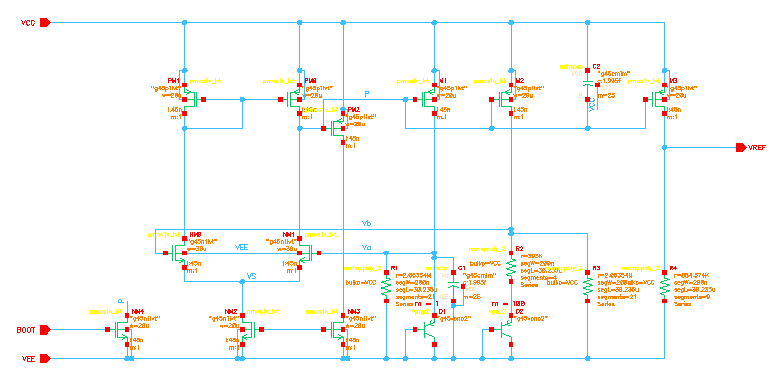
\includegraphics[width=\columnwidth]{images/bg_prop.eps}
    \caption{Schematic of proposed bandgap in C\=adence Virtuoso.} \label{fig:cadence_prop} 
\end{figure}

While threshold parameters for the process used were given, it may have also been useful to indicate certain parameters for the vertical BJTs used as quasi-diodes for the process used, since typical doping profiles and junction areas will have a fundamental impact on the bandgap performance. Likewise, since the resistors used in this design are fabricated from the n-type diffusion layer, they will have a temperature coefficient that is interdependent with the bipolar and MOS devices of the process, which is typically a known value, and could have been stated in some way.

Something of note is that the original presentation of the \(V_{ref}\) equations in the paper leaves something to be desired for allowing the reader to easily draw connections between the designs compared in the paper. Care has been taken to rewrite them here in such a manner.

\section{Recommendations}

Based on the stated critiques, a first course of action to truly verify this design's performance could be to construct it in a process that is designed with low voltage operation in mind, where threshold voltages closer to those used in their simulated version would allow truly sub-\qty{1}{\V} \(V_{CC}\) operation. The same number of data points should be used in reporting distribution data from the new and conventional designs, or reasoning should be given for why there is a difference in number. 

The reliance on a ratio of resistance in the proposed design does not lend well to the process variation of resistors created in standard CMOS processes. The values used in circuit are large and would not be easily created in a polysilicon layer with reduced temperature coefficient from the n-implant layer. Possible options may be to use a process that can implement low-tempco thin film resistors, use trimmed resistor networks, and even integrate these with trimmed BJT networks to further correct the temperature curve~\cite{Brokaw1974,Malcovati2001,Mok2004}. Another option is to forego the use of resistors entirely and utilize subthreshold MOS devices as resistive elements to leverage their temperature coefficient. This has an additional advantage of reduced coupled noise while retaining CMOS compatibility~\cite{Buck2002}. Switched capacitor designs, while offering better ratio matching in CMOS processes than resistive networks, must be carefully implemented to avoid noise injection into the reference circuit.

Recently, the idea of using native CMOS devices with low threshold has been adapted to a fully-CMOS based design, with switched-capacitor offset cancellation and additional noise suppression, achieving a lower \(V_{CC}\) limit of \qty{0.5}{\V}~\cite{Ria2021}. This design is robust with a temperature coefficient of \qty{45}{\ppm\per\degree\C} over 10-\qty{50}{\degree\C} shown after construction in a \qty{180}{\nm} process. In the future, precision trimming applied to this circuit may further increase its precision.

\section{Conclusion}

The bandgap reference design proposed by Banba et al. in 1998 has served as the basis for countless modifications of the circuit in an attempt to adapt it to lower supply voltages. Its impact on the industry is irrefutable with over 800 collective citations for the two original publications, which will likely continue to grow as the push to squeeze as much power savings as possible out of CMOS processes increases. The original publications leave something to be desired from the presented validation of the circuit design, by constructing the circuit in a process that was not only not designed for low voltage operation and did not reflect the simulated process parameters, but completely prevented the design from being validated under the conditions for which it was designed. The robustness of the Toshiba engineers' approach has been well-proven in literature since their publication, but it is conceivable that the impact of this design may have been further increased by presenting hardware data that supported its goals.




% An example of a floating figure using the graphicx package.
% Note that \label must occur AFTER (or within) \caption.
% For figures, \caption should occur after the \includegraphics.
% Note that IEEEtran v1.7 and later has special internal code that
% is designed to preserve the operation of \label within \caption
% even when the captionsoff option is in effect. However, because
% of issues like this, it may be the safest practice to put all your
% \label just after \caption rather than within \caption{}.
%
% Reminder: the "draftcls" or "draftclsnofoot", not "draft", class
% option should be used if it is desired that the figures are to be
% displayed while in draft mode.
%
%\begin{figure}[!t]
%\centering
%\includegraphics[width=2.5in]{myfigure}
% where an .eps filename suffix will be assumed under latex, 
% and a .pdf suffix will be assumed for pdflatex; or what has been declared
% via \DeclareGraphicsExtensions.
%\caption{Simulation results for the network.}
%\label{fig_sim}
%\end{figure}

% Note that the IEEE typically puts floats only at the top, even when this
% results in a large percentage of a column being occupied by floats.


% An example of a double column floating figure using two subfigures.
% (The subfig.sty package must be loaded for this to work.)
% The subfigure \label commands are set within each subfloat command,
% and the \label for the overall figure must come after \caption.
% \hfil is used as a separator to get equal spacing.
% Watch out that the combined width of all the subfigures on a 
% line do not exceed the text width or a line break will occur.
%
%\begin{figure*}[!t]
%\centering
%\subfloat[Case I]{\includegraphics[width=2.5in]{box}%
%\label{fig_first_case}}
%\hfil
%\subfloat[Case II]{\includegraphics[width=2.5in]{box}%
%\label{fig_second_case}}
%\caption{Simulation results for the network.}
%\label{fig_sim}
%\end{figure*}
%
% Note that often IEEE papers with subfigures do not employ subfigure
% captions (using the optional argument to \subfloat[]), but instead will
% reference/describe all of them (a), (b), etc., within the main caption.
% Be aware that for subfig.sty to generate the (a), (b), etc., subfigure
% labels, the optional argument to \subfloat must be present. If a
% subcaption is not desired, just leave its contents blank,
% e.g., \subfloat[].


% An example of a floating table. Note that, for IEEE style tables, the
% \caption command should come BEFORE the table and, given that table
% captions serve much like titles, are usually capitalized except for words
% such as a, an, and, as, at, but, by, for, in, nor, of, on, or, the, to
% and up, which are usually not capitalized unless they are the first or
% last word of the caption. Table text will default to \footnotesize as
% the IEEE normally uses this smaller font for tables.
% The \label must come after \caption as always.
%
%\begin{table}[!t]
%% increase table row spacing, adjust to taste
%\renewcommand{\arraystretch}{1.3}
% if using array.sty, it might be a good idea to tweak the value of
% \extrarowheight as needed to properly center the text within the cells
%\caption{An Example of a Table}
%\label{table_example}
%\centering
%% Some packages, such as MDW tools, offer better commands for making tables
%% than the plain LaTeX2e tabular which is used here.
%\begin{tabular}{|c||c|}
%\hline
%One & Two\\
%\hline
%Three & Four\\
%\hline
%\end{tabular}
%\end{table}


% Note that the IEEE does not put floats in the very first column
% - or typically anywhere on the first page for that matter. Also,
% in-text middle ("here") positioning is typically not used, but it
% is allowed and encouraged for Computer Society conferences (but
% not Computer Society journals). Most IEEE journals/conferences use
% top floats exclusively. 
% Note that, LaTeX2e, unlike IEEE journals/conferences, places
% footnotes above bottom floats. This can be corrected via the
% \fnbelowfloat command of the stfloats package.


% if have a single appendix:
%\appendix[Proof of the Zonklar Equations]
% or
%\appendix  % for no appendix heading
% do not use \section anymore after \appendix, only \section*
% is possibly needed

% use appendices with more than one appendix
% then use \section to start each appendix
% you must declare a \section before using any
% \subsection or using \label (\appendices by itself
% starts a section numbered zero.)
%


% \appendices
% \section{Proof of the First Zonklar Equation}
% Appendix one text goes here.

% % you can choose not to have a title for an appendix
% % if you want by leaving the argument blank
% \section{}
% Appendix two text goes here.


% use section* for acknowledgment
\section*{Acknowledgment}

The author would like to thank Dr. Mark Pude for providing the paper to be analyzed in his course \emph{Mixed-Signal IC Design} at Rochester Institute of Technology.


% Can use something like this to put references on a page
% by themselves when using endfloat and the captionsoff option.
\ifCLASSOPTIONcaptionsoff
  \newpage
\fi



% trigger a \newpage just before the given reference
% number - used to balance the columns on the last page
% adjust value as needed - may need to be readjusted if
% the document is modified later
%\IEEEtriggeratref{8}
% The "triggered" command can be changed if desired:
%\IEEEtriggercmd{\enlargethispage{-5in}}

% references section

% can use a bibliography generated by BibTeX as a .bbl file
% BibTeX documentation can be easily obtained at:
% http://mirror.ctan.org/biblio/bibtex/contrib/doc/
% The IEEEtran BibTeX style support page is at:
% http://www.michaelshell.org/tex/ieeetran/bibtex/
%\bibliographystyle{IEEEtran}
% argument is your BibTeX string definitions and bibliography database(s)
%\bibliography{IEEEabrv,../bib/paper}
%
% <OR> manually copy in the resultant .bbl file
% set second argument of \begin to the number of references
% (used to reserve space for the reference number labels box)


\bibliographystyle{IEEEtranDOI}
\bibliography{main}


% biography section
% 
% If you have an EPS/PDF photo (graphicx package needed) extra braces are
% needed around the contents of the optional argument to biography to prevent
% the LaTeX parser from getting confused when it sees the complicated
% \includegraphics command within an optional argument. (You could create
% your own custom macro containing the \includegraphics command to make things
% simpler here.)
%\begin{IEEEbiography}[{\includegraphics[width=1in,height=1.25in,clip,keepaspectratio]{mshell}}]{Michael Shell}
% or if you just want to reserve a space for a photo:


% if you will not have a photo at all:
% \begin{IEEEbiographynophoto}{Chris Biancone}
% Biography text here.
% \end{IEEEbiographynophoto}


% insert where needed to balance the two columns on the last page with
% biographies
%\newpage


% You can push biographies down or up by placing
% a \vfill before or after them. The appropriate
% use of \vfill depends on what kind of text is
% on the last page and whether or not the columns
% are being equalized.

%\vfill

% Can be used to pull up biographies so that the bottom of the last one
% is flush with the other column.
%\enlargethispage{-5in}



% that's all folks
\end{document}


